\subsection{Limits for multiplicities}
    Considering difference multisets over an arbirary loop (quasigroup with an identity) one can notice that some of the surfaces defined by our equations are always the same. There is always the hyperplane $\sum {n_i} = k$ and the hypersphere $\sum n_i^2 = k + \lambda$ centered at the origin (see figure \ref{general:figure:surfaces}). You could notice right away that the second equation confines every multiplicity: $n_i \leq \sqrt{k+\lambda}$. By investigating the intersection more thoroughly we may discover that the multiplicities are actually bound to be near (in a sense) to their average---$k/v$.

    \begin{figure}
        \centering
        \begin{subfigure}[b]{0.5\textwidth}
            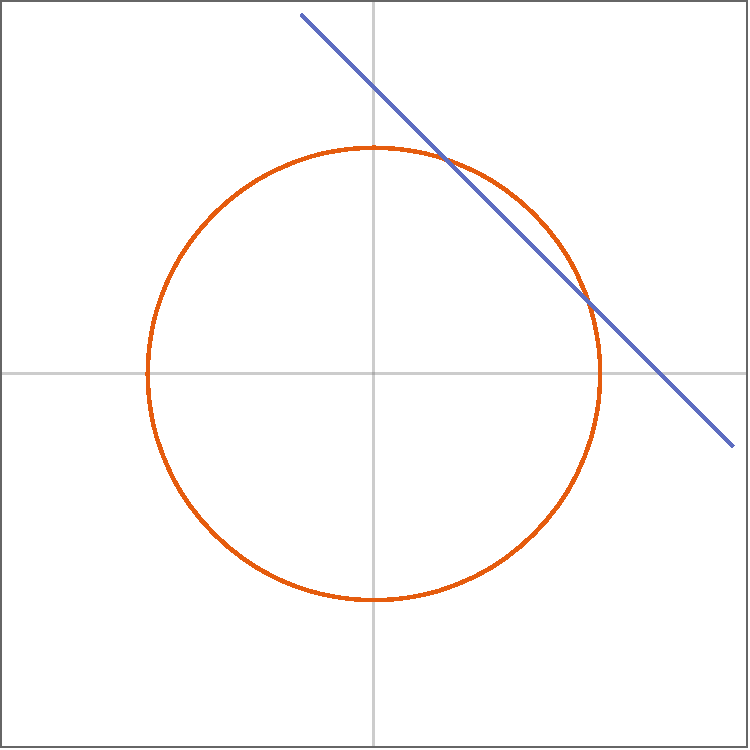
\includegraphics[width=\textwidth]{assets/surfacesIn2D}
        \end{subfigure}%
        ~
        \begin{subfigure}[b]{0.5\textwidth}
            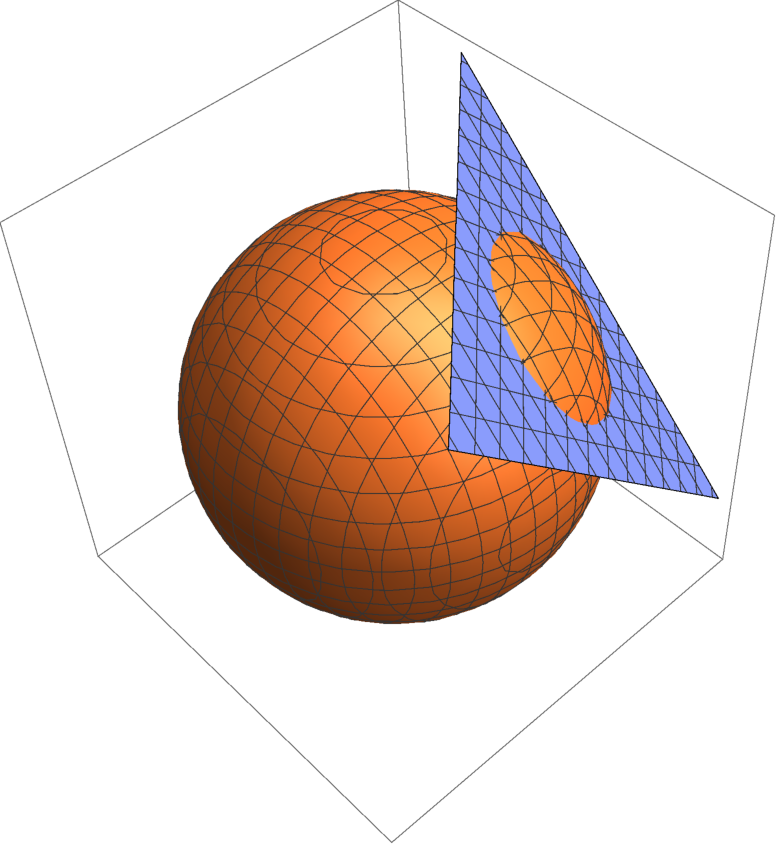
\includegraphics[width=\textwidth]{assets/surfacesIn3D}
        \end{subfigure}
        \caption{The $\sum {n_i} = k$ and $\sum n_i^2 = k + \lambda$ surfaces in two and three dimensions.}
        \label{general:figure:surfaces}
    \end{figure}
        
    \begin{theorem}
        \label{general:theorem:limits}
        If $M$ is a $(Q,k)$-difference multiset then
        \begin{equation}
            \forall q \in Q \colon \frac{k-(v-1)\sqrt k}{v} \leq n(q,M) \leq \frac{k+(v-1)\sqrt k}{v}
        \end{equation}
    \end{theorem}
    
    \begin{proof}
        Take \eqref{apparatus:eq:system} for the identity element and \eqref{apparatus:eq:ni} as constraints.
        
        \begin{equation}
            \begin{cases}
                \sum {n_i} = k \\
                \sum (n_i(n_{i}-1)) = \lambda
            \end{cases}
        \end{equation}
        
        Let's optimize $n_q$ respecting the constraints. We can add the first equation to the other to simplify the latter expression and let's also put all the terms on one side as follows.
        
        \begin{equation}
            \begin{cases}
                k - \sum {n_i} = 0 \\
                k + \lambda - \sum n_i^2 = 0
            \end{cases}
        \end{equation}
        
        We may now use a common optimization technique -- Lagrange multipliers to obtain the maximum and minimum of $n_q$ honoring the constraints by using the following Lagrange function (note that Lagranage multipliers $\lambda_1$ and $\lambda_2$ are notated per tradition and have nothing in common with the parameter $\lambda$).
        
        \begin{equation}
            \mathcal L = n_q - \lambda_1 (k - \sum n_i) - \lambda_2 (k + \lambda - \sum n_i^2)
        \end{equation}
        
        This gives the stated boundaries for any $n_q$ in a difference multiset. The optimization calculations are not included as those are tedious and in no way novel.
    \end{proof}

    Theorem \ref{general:theorem:limits} might appear uninspiring at first but it not only suggests using digressions instead of multiplicities (thus simplifying the equations) but also greatly reduces the amount of options for every $n_q$. This simplification is a crucial stepping stone in making decent computer searches possible which allowed us to discover some of the patterns that lead to results presented in this paper.
        
    \begin{figure}
        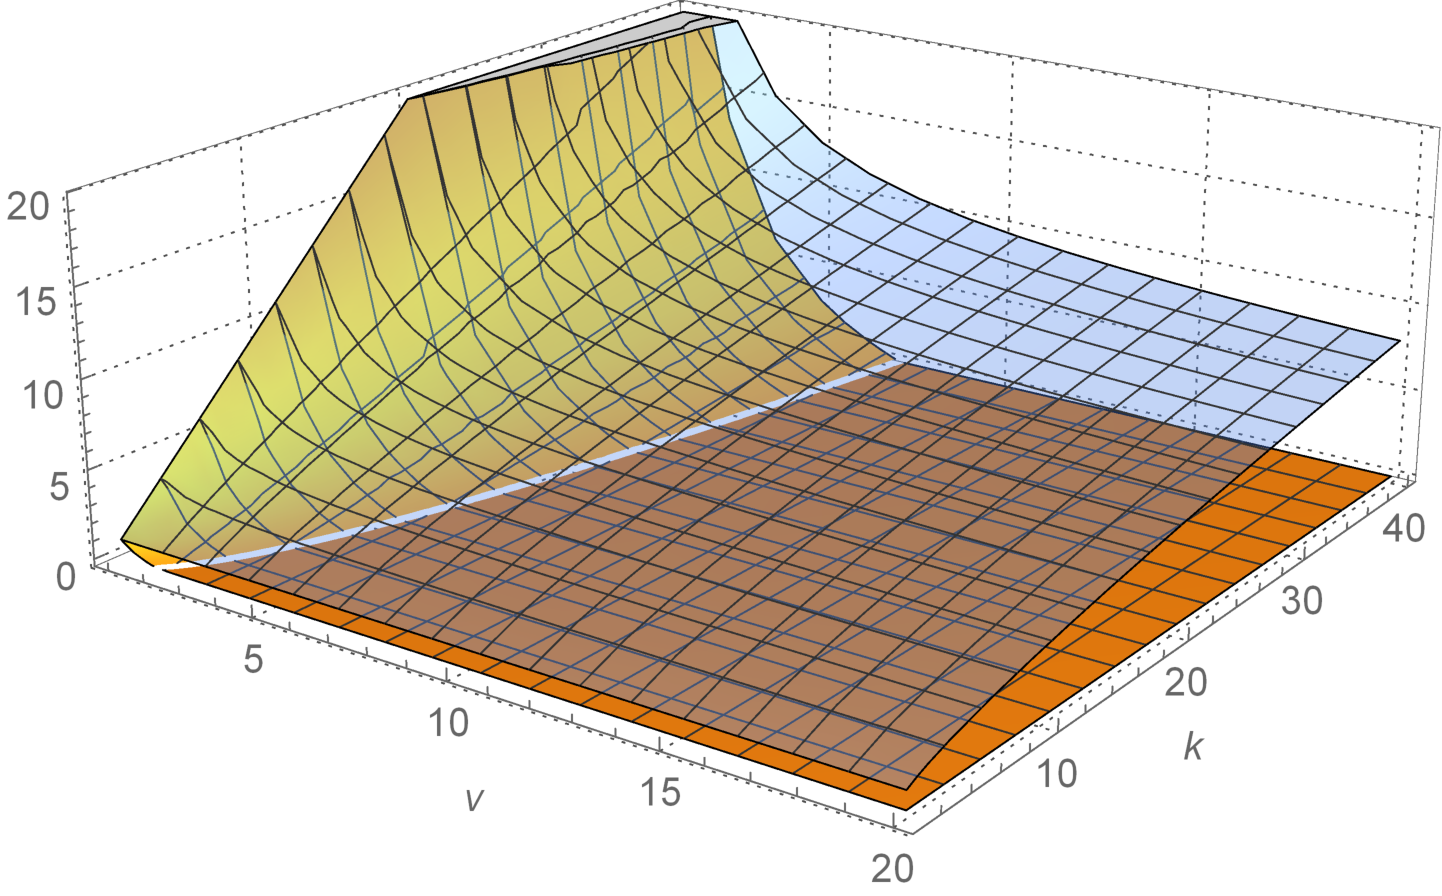
\includegraphics[width=\textwidth]{assets/boundingSurfaces}
        \caption{Lower and upper limits for the values of $n_q$ with respect to $v$ and $k$.}
        \label{general:figure:limits}
    \end{figure}
    
\subsection{A family of difference multisets for every quasigroup}
    Based on particular results discussed further, we have discovered a construction that works whenever $k$ is close to a multiple of $v$.
    
    \begin{theorem}
        \label{regular:theorem:regular}
        $(Q,k)$-difference multiset exists if $v \mid \sqrt k$ or $\sqrt k \equiv \pm 1 \mod v$ and it's digressions are 
            \begin{itemize}
                \item If $\sqrt k \equiv 1 \mod v$ then $d_i = v-1$ for any element $i$ and $d_{j \neq i} = -1$ for the other elements.
                \item If $\sqrt k \equiv -1 \mod v$ then $d_i =1-v$ for any element $i$ and $d_{j \neq i} = 1$ for the other elements.
                \item Both of the above if $v \mid \sqrt k$.
            \end{itemize}
    \end{theorem}
    
    \begin{proof}
        The conditions in theorem guarantees the multiplicities to be integers. All that is left is to demonstrate that they actually make up a difference multiset.
        
        Considering \eqref{apparatus:eq:dsystem} for non-identity elements we can notice that a any particular multiplicity will be involved in two of the products---once as $i$ and once as $i+q$ (but not both at the same time as we consider non-identity $q$ now). Other $v-2$ products are destined to contain other multiplicities solely which leads us to true equation.
        
        \begin{equation}
            \sum d_i d_{i+q} = -2(v-1) + (v-2) = -v
        \end{equation}

        In case we're dealing with a loop, we must consider the case of $q$ being the identity which is also shown to be true.
        
        \begin{equation}
            \sum d_i^2  = \left( \pm (v-1) \right)^2 + (v-1) \left( \mp 1 \right)^2 = v^2 - v
        \end{equation}
    
        It is straightforward to check that \eqref{apparatus:eq:di} turns out true as well.
    \end{proof}

\subsection{Difference multisets for cyclic groups}
    For cyclic matrices we can write \eqref{apparatus:eq:dsystem} as
    \begin{equation}
        D d = \bf v
    \end{equation}\
    where $d = (d_0, d_1, \ldots, d_{v-1})$, $D_{ij} = d_{i+j}$ and $\bf v = (v^2-v, -v, -v, \ldots)$.
    
    The form of the matrix $D$ is the following:
    \begin{equation}
        \label{general:eq:anticirculant_matrix}
        D =
        \begin{pmatrix}
            d_0 & d_1 & d_2 & \cdots & d_{v-1} \\ 
            d_1 & d_2 & d_3 & \cdots & d_0 \\
            d_2 & d_3 & d_4 & \cdots & d_1 \\
            \vdots & \vdots & \vdots & \ddots & \vdots \\
            d_{v-2} & d_{v-1} & d_0 & \cdots & d_{v-3} \\
            d_{v-1} & d_0 & d_1 & \cdots & d_{v-2} \\
        \end{pmatrix}
    \end{equation}
    
    This is a special case of Hankel matrix sometimes called \emph{anticirculant matrix}. The structure of the corresponding $D$ will be the same.
    
    \subsubsection{Solving equations with anticirculant matrices}
    \label{general:sec:anticirculant}
        We weren't able to track down a source dealing with matrices like \eqref{general:eq:anticirculant_matrix}, however we managed to apply the same methods as with circulant matrices \cite{wiki:circulant_matrix}.
        
        Let's consider the equation $Ax=b$ with an anticirculant $v \times v$ matrix
        \begin{equation}
            A =
            \begin{pmatrix}
                a_0 & a_1 & a_2 & \cdots & a_{v-1} \\ 
                a_1 & a_2 & a_3 & \cdots & a_0 \\
                a_2 & a_3 & a_4 & \cdots & a_1 \\
                \vdots & \vdots & \vdots & \ddots & \vdots \\
            \end{pmatrix}
        \end{equation}\
        and a vector $b=(b_0, b_1, b_2, \vdots)^T$. 
        
        Denote $a=(a_1,\ldots,a_{v-1})$. We can now express the equation row by row (please consider indices $\mod v$):
        \begin{equation}
            b_j = \sum_{k=0}^{v-1} a_{j+k} x_k
        \end{equation}
        
        Apply discrete Fourier transform:
        \begin{equation}
            \mathcal{F} (b)_m = \sum_{j=0}^{v-1} b_j \exp(-2\pi i \frac{jm}v )
        \end{equation}
        
        Insert $b_j$ obtaining
        \begin{equation}
        \begin{split}
            \mathcal{F} (b)_m
            &= \sum_{j=0}^{v-1} \sum_{k=0}^{v-1} a_{j+k} x_k \exp(-2\pi i \frac{jm}v) \\
            &= \sum_{j=0}^{v-1} \sum_{k=0}^{v-1} x_k \exp(2\pi i \frac{km}v) a_{j+k} \exp(-2\pi i \frac{(j+k)m}v)  \\
            &= \sum_{k=0}^{v-1} x_k \exp(2\pi i \frac{km}v) \sum_{j'=k}^{v+k-1} a_{j'} \exp(-2\pi i \frac{j'm}v)
        \end{split}
        \end{equation}
        
        Looking at the inner sum we should note that not only we take indices $\mod v$ but the $j'$ in the exponent can be taken $\mod v$ as well. Let's use $j'' = j' \mod v$.
        \begin{equation}
            \sum_{j'=k}^{v+k-1} a_{j'} \exp(-2\pi i \frac{j'm}v) = 
            \sum_{j''=0}^{v-1} a_{j''} \exp(-2\pi i \frac{j''m}v) = \mathcal{F}(a)_m
        \end{equation}
        
        We can now finish the transformation:
        \begin{equation}
        \begin{split}
            \mathcal{F} (b)_m
            &= \sum_{k=0}^{v-1} x_k \exp(2\pi i \frac{km}v) \mathcal{F}(a)_m \\
            &= \mathcal{F}(a)_m (\sum_{k=0}^{v-1} x^*_k \exp(-2\pi i \frac{km}v))^* \\
            &= \mathcal{F}(a)_m \mathcal{F}^*(x^*)_m 
            = v \mathcal{F}(a)_m \mathcal{F}^{-1}(x)_m
        \end{split}
        \end{equation}
        
        The final form (exploiting the Fourier transform property $\mathcal{F}^{-1}(x) = \mathcal{F}^*(x^*)/v$) was included for completeness as it allows to explicitly express $x = \mathcal{F} \left(\frac1v \frac{\mathcal{F}(b)}{\mathcal{F}(a)} \right)$. However, we will use $\mathcal{F} (b)_m = \mathcal{F}(a)_m \mathcal{F}^*(x^*)_m$.
    
    \subsubsection{Solving the digression equation}
        The $D$ and $d$ in equation $Dd=\bf v$ is linked in the same way as $A$ and $a$ in section \ref{general:sec:anticirculant}. The image of $Dd=\bf v$ is
        
        \begin{equation}
            \mathcal{F} ({\bf v})_m = \mathcal{F}(d)_m \mathcal{F^*}(d^*)_m
        \end{equation}

        As we are only interested in real $d$, we can even simplify it to
        
        \begin{equation}
            \label{general:eq:dfourier}
            \mathcal{F} ({\bf v})_m = \mathcal{F}(d)_m \mathcal{F^*}(d)_m = |\mathcal{F}(d)_m|^2
        \end{equation}
        
        Remembering ${\bf v} = (v^2-v, -v, -v, \ldots)$ we can find that $\mathcal{F}({\bf v'}) = (0,v^2,v^2,\ldots)$ and \eqref{general:eq:dfourier} becomes
        \begin{equation}
            \label{gen:eq:dfourierfinal}
            \left| \sum_{j=0}^{v-1} d_j \exp(-2\pi i \frac{jm}v) \right| = v (1-\delta_{m0})
        \end{equation}

        For any $m | v$ we can note that $\delta_{m0}=0$ and
        \begin{equation}
            \label{general:eq:split_fourier}
            \left| \sum_{j=0}^{v-1} d_j e^{\frac{-2\pi i m j}v} \right|
            = \left| \sum_{j=0}^{v/m-1} \sum_{k=0}^{m-1}  d_{j+kv/m} e^{\frac{-2\pi i m j}v} \right|
            =v
        \end{equation}\
        as 
        \begin{equation}
            e^{\frac{-2\pi i m (j+kv/m)}v} = e^{\frac{-2\pi i m j}v} e^{-2\pi i k} = e^{\frac{-2\pi i m j}v}
        \end{equation}
        
        We consider expressions \eqref{gen:eq:dfourierfinal} and \eqref{general:eq:split_fourier} as the main results of this section, here's how one can use it.
        
        \begin{proposition}
            \label{general:theorem:even_cyclic}
            In cyclic groups of even cardinality $\sum_{k=0}^{v/2-1} d_{2k} = \pm \frac v2$ and $\sum_{k=0}^{v/2-1} d_{2k+1} = \mp \frac v2$.
        \end{proposition}
        \begin{proof}
            Take \eqref{general:eq:split_fourier} for $m=v/2$
            \begin{equation}
                \left| \sum_{k=0}^{v/2-1} d_{2k} - \sum_{k=0}^{v/2-1} d_{2k+1} \right| = v
            \end{equation}
            
            We've split $d$ in half and got that total of one half is by $v$ larger than the total of the other half. The statement of the theorem follows as soon as we remember the grand total $\sum d_i = 0$.
        \end{proof}
        
        \begin{remark}
            Similar relation also holds true for some (many? all?) other structures that are not cyclic groups. For example in $\mathbb Z_2 \times \mathbb Z_2$ with elements $\set{i,j,k,l}$ in any order we have $d_i+d+j-(d_k+d_l)=\pm 4$.
        \end{remark}


\subsection{Difference multisets over $\mathbb Z_2^n$}
    \label{sec:z2n}
    We obtained a construction that produces plenty of difference multisets in $\mathbb Z_2^n$. We shall start by explaining the construction and then a proof and analysis of the construction will be presented.

    \subsubsection{Construction}
        Consider the elements $i \in \mathbb Z_2^n$ as n-tuples $i=(i_1, \ldots, i_n)$.
        
        Select a hyperplane $H_1$ out of $\mathbb Z_2^n$ defined by equation $0 = a_0 + a_1 i_1 + a_2 i_2 + \ldots + a_n i_n$ ($0=a_0+a\cdot i$) with $a_k \neq 0$ for at least one $k \neq 0$. Set $d_h = -1$ for every $h \in H_1$.
        
        As for the remaining $(n-1)$-dimensional halfspace: take a hyperplane $H_2$ out of this and set $d_h = 3$ for every $h \in H_2$.
        
        Repeat this process $0 \leq m \leq n-1$ times setting $d_h = \sum\limits_{j=0}^k (-2)^j$ for every $h \in H_k$.
        
        You will end up with the final subspace $H_f$ remaining. Select an element $e$ and set $d_e = (-1)^m v + \sum\limits_{j=0}^{m+1} (-2)^j$. Set $d_h = \sum\limits_{j=0}^{m+1} (-2)^j$ for the remaining $h \in H_f$.
        
        One can also flip the sign on every $d_i$ getting another bunch of difference multisets.
        
    \subsubsection{A few examples}
        
        \begin{example}
            Take $n=7$. Thus $v=2^n=128$. Take hyperplane $H_1$ defined by $0=i_1$, and set $d_h=-1$ for all $h\in H_1$ i.e. set $d_{0000000}=d_{0000001}=\ldots=d_{0111111}=-1$.
            
            Let's continue with the remaining subspace ($0=1+i_1$). Select another halfpace $H_2$ defined by $0=i_2$ and set $d_{1000000}=\ldots=d_{1011111}=3$.
            
            Let's choose $m=4$. We must then repeat the bisections two more times setting $d_h=-5$ for $h\in H_3$ and $d_h=11$ for $h \in H_4$.
            
            We have 8 elements left. Let's set $d_{1111111} = (-1)^{m} v + \sum\limits_{j=0}^{m+1} (-2)^j = v - 21 = 107$ and it remains that the other $d_{1111000}=\ldots=d_{1111110}=-21$.
        \end{example}
        
        For tighter examples (with $m\geq n-2$) the multiplicity of the final element will take form of $\sum (-2)^j$ as well. All the digressions will appear to be on the sequence $-1,3,-5,11,-21,43,-85,\ldots$ \cite{A077925}.
        
        \begin{example}
          Take $n=4$ and $m=2$. You will have eight $d_i=-1$, four $d_i=3$, three $d_i=-5$ and one $d_i=11$.
        \end{example}
        
        \begin{example}
            \label{2n:example:edge}
            Let's take $n=4$ and $m=3$. You get half the digressions (eight) $d_i=-1$. You set another quarter---four digressions $d_i=3$. Then you set two $d_i=-5$. Halfspace with two elements remains. All except one are set to $d_i=11$. And the last one is $-v+11=-5$ Thus you end up with the same set of digressions as in the previous example.
        \end{example}

        Example \ref{2n:example:edge} shows that some of the constructions (the ones with $m=n-1$) produce a difference multiset that coincides with the $m=n-2$ construction.
    
    \subsubsection{Proof}
        For a selected $0 \leq m \leq n-1$ this construction provides us with $2^{n-k}$ digressions of value $d_h=\sum\limits_{j=0}^k(-2)^j$ for each $1<k\leq m$ (none of these if $m=0$), $2^{n-m}-1$ digressions equal to $\sum\limits_{j=0}^{m+1}(-2)^j$ and one digression equal to $(-1)^m 2^n+\sum\limits_{j=0}^{m+1}(-2)^j$.
        
        Checking equation $\sum d_i = 0$ and $\sum d_i^2 = v(v-1)$ is straightforward if you take into account that $\sum\limits_{j=0}^k(-2)^j=(1-(-2)^{k+1})/3$.
        
        Equations \eqref{apparatus:eq:dsystem} are left to check. We began the construction by selecting a hyperplane $H_1$ defined by $0=a_0+a\cdot i$ where $a=(a_,a_2,\ldots)$ and $i=(i_1,i_2,\ldots)$ Depending on selection of $q=(q_1,q_2,\ldots)$ there are two cases:
        \begin{itemize}
            \item If $1 \equiv a\cdot q \mod 2$ then $\forall i \in H_1 : i+q \notin H1 $ and $\forall i \notin H_1 : i+q \in H1$;
            \item If $0 \equiv a\cdot q \mod 2$ then $\forall i \in H_1 : i+q \in H1 $ and $\forall i \notin H_1 : i+q \notin H1$.
        \end{itemize}
        
        In the first case every $d_i d_{i+q}$ involves factor $-1$. $\sum d_i d_{i+q} = -2\sum\limits_{i\notin H_1} d_i = -2 (\sum d_i - \frac v2 (-1)) = -v$.
        
        In the second case $d_i d_{i+q} = 1$ for every $i \in H_1$ and $\sum\limits_{i \in H_1} d_i d_{i+q} = \frac v2$. So the remaining stuff must make up $-\frac {3v}2$ For the remaining stuff we are once again split into two cases depending on $q$ and the initial choice of $H_2$. Either both $i$ and $i+q$ belong to the different sub-hyperplanes for every $i$, or they belong to the same for every $i$. That is, we either have $\sum\limits_{j=0}^2 (-2)^j = 3$ in every factor or we continue the process.
        
        In general for any $q$ we will end up at some step where we will have already summed up $d_i^2$ for $i \in H_1 \cup H_2 \cup \ldots \cup H_r$ and at the next step we will have one of these cases:
        
        \begin{itemize}
            \item No more $H_{r+1}$ has been constructed---only $2^{n-r}-1$ elements with $d_i = \sum\limits_{j=0}^{r+1} (-2)^j$ and a single $d_e = (-1)^m 2^n + \sum\limits_{j=0}^{r+1} (-2)^j$;
            \item $i \in H_{r+1}$ will have to be multiplied with the items outside $H_{r+1}$ (like the first case in the previous fork).
        \end{itemize}

        The first case checks out:
        \begin{equation}
            \begin{split}
                \sum d_i^2 & \\
                = & \sum\limits_{H_1 \cup \ldots \cup H_r} d_i^2 \\
                & + (2^{n-r}-2) \left(\sum\limits_{j=0}^{r+1} (-2)^j \right)^2 \\
                & + 2 \left(\sum\limits_{j=0}^{r+1} (-2)^j \right) \left( (-1)^r 2^n + \sum\limits_{j=0}^{r+1} (-2)^j \right) \\
                = & - 2^n = -v
            \end{split}
        \end{equation}
    
        The second does as well:
        \begin{equation}
            \begin{split}
                \sum d_i^2 & \\
                = & \sum\limits_{H_1 \cup \ldots \cup H_r} d_i^2 \\
                + & 2 \left(\sum\limits_{j=0}^{r+1} (-2)^j \right) 
                 \Bigg(
                    \sum\limits_{k=r+2}^{m} 2^{n-k} \sum\limits_{j=0}^k (-2)^j \\
                   & + (2^{n-m}-1)\sum\limits_{j=0}^{m+1} (-2)^j \\
                   & + (-1)^m 2^n + \sum\limits_{j=0}^{m+1} (-2)^j
                 \Bigg) \\
                = & - 2^n = -v
            \end{split}
        \end{equation}
    
    \subsubsection{Analysis}
        For $n \leq 3$ the construction makes all the difference multisets there are. This can be shown explicitly by solving the digression equations.
        
        We don't know about larger groups. Our construction produces $2^n$ different values for $n \leq 3$ but only 12, 16 and 20 different $d_i$ values for $n$ of 4,5 and 6 respectively.
        
        As for the number of difference multisets, this construction produces
        \begin{equation}
            2 \sum\limits_{j=2}^n 2^j \prod\limits_{k=j+1}^n (2^{k+1}-2)
        \end{equation}\
        solutions for $d_i$ over $\mathbb Z_2^n$. The counting argument is that we can select $H_1$ in $2^{n+1}-2$ ways, $H_2$ in $2^n-2$ etc. until you stop and choose one of the remaining $2^j$ elements. And twice everything as you can flip the signs.
        
        The difference multisets (i.e. integer solutions $n_i=\frac{k+d_i \sqrt k}v$) themselves are produced whenever $v | \sqrt k$. In addition the cases of single $d_e = \pm (v-1)$ and the rest $d_i = \mp 1$ we get integer $n_i$ for $v \equiv \mp 1 \mod v$.
        
\section{Difference multisets over the three element group}
    \label{sec:z3}
    There is only one group of three elements. Let's take it in form of $\mathbb Z_3$. What must the $k$ be for $(\mathbb Z_3,k)$-difference multiset to exist? What are these difference multisets and how many of them are there for a particular value of $k$?

    To answer these questions we shall write down \eqref{apparatus:eq:system} for a non-identity element and combine it with \eqref{apparatus:eq:ni} and \eqref{apparatus:eq:parameters} to form a system of equations.

    \begin{equation}
        \label{v3:eq:constraints}
        \begin{cases}
            3\lambda = k(k-1) \\
            \sum n_i = k \\
            \sum n_i n_{i+1} = \lambda
        \end{cases}
    \end{equation}

    We may now combine the equations to discover a relation between multiplicities of elements.

    \begin{theorem}
        \label{v3:theorem:relations}
        Multiplicities of different $(\mathbb Z_3,k)$-difference multiset elements $i$ un $j$ are related via
        \begin{equation}
            \label{v3:eq:relations}
            n_{i\neq j} = \frac{k-n_j \pm \sqrt{\frac{4k-(k-3n_j)^2}{3}}}{2}
        \end{equation}
    \end{theorem}

    \begin{proof}
        Take any element $\gamma \in \mathbb Z_3$ and assign $c = n_\gamma$. Let's use $\alpha$ and $\beta$ to name the remaining elements of $\mathbb Z_3$. The system \eqref{v3:eq:constraints} can now be rewritten:
        \begin{equation}
            \begin{cases}
                n_\alpha + n_\beta = k - c \\
                n_\alpha n_\beta + c (n_\alpha + n_\beta)  = \lambda 
            \end{cases}
        \end{equation}
        
        Substitute $k'=k-c$ and $\lambda' = \lambda + c^2-kc$ to obtain
        
        \begin{equation}
            \begin{cases}
                n_\alpha + n_\beta = k' \\
                n_\alpha n_\beta = \lambda'
            \end{cases}
        \end{equation}
        
        Eliminating $n_\beta$ we arrive at a quadratic equation that is solved into
        
        \begin{equation}
            n_\alpha = \frac{k' \pm \sqrt{k'^2-4\lambda'}}{2}
        \end{equation}
        
        Undo the substitutions and you're done.
    \end{proof}

    Considering the multiplicities in form of $n_i = \frac{k+\Delta_i}{3}$, we can restate \eqref{v3:eq:relations} into the following.

    \begin{equation}
        \label{v3:eq:relations_delta}
        n_{i\neq j} = \frac{k-n_j \pm \sqrt{\frac{4k-\Delta_j^2}{3}}}{2}
    \end{equation}

    The rest of analysis focuses on the $\Delta_i$ and it's effect on the above equation. The behaviour of expression under the root is tied to a topic in number theory called Löschian numbers \cite{oeisA003136}. These numbers make an appearance in a variety of fields (see comments in \cite{oeisA003136}).

    \begin{definition}
        \label{v3:def:loeshian}
        Number $k$ is called a Löschian number if $\exists a,b \in \mathbb Z \colon a^2+ab+b^2=k$.
    \end{definition}

    For our purposes (to eliminate unnecessary symmetries) we will only consider $a,b$ such that $a \geq b \geq 0$. This, however, doesn't change the scope of Löschian numbers.

    \begin{lemma}
        \label{v3:lemma:loeschian}
        For any Löschian number $k$ we can find $a,b \in \mathbb Z$ such that $a^2+ab+b^2=k$ and $a \geq b \geq 0$.
    \end{lemma}

    \begin{proof}
        As $k$ is a Löschian number there are $a',b' \colon a'^2+a'b'+b'^2=k$. We can construct $a,b$ such that $a^2+ab+b^2=k$ and $a \geq b \geq 0$ as follows:
        \begin{itemize}
            \item If $a' \geq 0$ and $b' \geq 0$ just take $a=a'$ and $b=b'$ or swap them if $a'<b'$.
            \item If $a'<0,b'<0$ take $a'=-a,b'=-b$ or swap them if $a'>b'$.
            \item If $ab<0$ take either $a'=|a|, b'=|a+b|$ or $a'=|a+b|, b'=|b|$. Swap places as necessary to ensure $a \geq b \geq 0$.
        \end{itemize}
    \end{proof}

    Having introduced the term, we may now introduce the promised link.

    \begin{lemma}
        \label{v3:lemma:square}
        There exists a $\Delta$ that makes $\frac{4k-\Delta^2}{3}$ a perfect square iff $k$ is Löschian number.
        
        $\Delta$ values that does the job are $\pm (2a+b), \pm (a+2b), \pm (a-b)$, where $a,b$ are such that $a \geq b \geq 0$ and $a^2+ab+b^2=k$. There is no other $\Delta$ that makes $\frac{4k-\Delta^2}{3}$ into square.
    \end{lemma}

    \begin{proof}
        For a Löschian number $k=a^2+ab+b^2$ take $\Delta$ equal to $\pm (2a+b)$, $\pm (a+2b)$ or $\pm (a-b)$ and obtain the value of expression in question to be $b^2$, $a^2$ or $(a+b)^2$ which are clearly squares.
        
        On the other hand, if $\frac{4k-\Delta^2}{3}$ is square, assign:
        \begin{equation}
            z^2 = \frac{4k-\Delta^2}{3}
        \end{equation}
        
        Rewrite
        \begin{equation}
            \frac{3z^2 + \Delta^2}{4} = k
        \end{equation}
        
        Noticing that $4$ divides $3z^2 + \Delta^2$ we can conclude that $z$ and $\Delta$ are of the same parity (because $z^2 \equiv \Delta^2 \mod 4$). Thus $2$ divides both $\Delta-z$ and $\Delta+z$.
        
        We can now find integers $a,b$ such that $a \geq b \geq 0$ and $a^2+ab+b^2=k$ (thus $k$ is a Löschian number) and the $\Delta$ can be expressed in one of the expressions stated in lemma.
        
        \begin{itemize}
            \item If $z \geq \Delta$ take $a=\frac{z+\Delta}{2}$ and $b=\frac{z-\Delta}{2}$. Then $a-b=\Delta$.
            \item If $\Delta \geq z \geq \frac \Delta 3$ take $a=z$ and $b=\frac{\Delta-z}{2}$. Then $a+2b=\Delta$.
            \item If $\frac \Delta 3 \geq z$ take $a=\frac{\Delta-z}{2}$ and $b=z$. Then $2a+b=\Delta$.
        \end{itemize}
    \end{proof}

    Let's introduce the following notation for the three values used in lemma \ref{v3:lemma:square}. The rest can be expressed as $-\Delta_i$:
    \begin{equation}
        \label{v3:eq:deltas}
        \Delta_\alpha = 2a+b, \Delta_\beta = -a-2b, \Delta_\gamma = -a+b
    \end{equation}

    These $\Delta_i$ will be used in the following theorem and $\alpha$, $\beta$ and $\gamma$ are labels that, as before, we use to label the elements of $\mathbb Z_3$ in arbitrary order. We can now state our main result which is both construction and existence criterion for $(\mathbb Z_3,k)$-difference multisets.

    \begin{theorem}
        \label{v3:theorem:loeschian}
        For every pair $a,b \in \mathbb Z$ such that $k=a^2+ab+b^2$ and $a \geq b \geq 0$ there are exactly $-(k+1) \mod 3$ (up to automorphisms) $(\mathbb Z_3,k)$-difference multisets and the multiplicities of their elements are
        
        \begin{itemize}
            \item $n_i=\frac{k+\Delta_i}{3}$ for one and $n_i=\frac{k-\Delta_i}{3}$ for the other if $3 \mid k$.
            \item $n_i=\frac{k+\Delta_i}{3}$ if $3 \nmid k$ un $b-a \equiv 1 \mod 3$.
            \item $n_i=\frac{k-\Delta_i}{3}$ if $3 \nmid k$ un $a-b \equiv 1 \mod 3$.
        \end{itemize}
    \end{theorem}

    \begin{proof}
        According to lemma \ref{v3:lemma:square}, the expression \eqref{v3:eq:relations_delta} will equal integer only if $k$ is a Löschian number and $\Delta_j$ is one of the listed on \eqref{v3:eq:deltas} or a negative of that.
        
        Insert the constructions listed in \eqref{v3:theorem:loeschian} into \eqref{v3:eq:relations} to check that these are indeed multiplicities that make up a difference multiset if the numbers are whole. One can also check that using $\Delta_\alpha$ to construct one of the multiplicities you will notice $\Delta_\beta$ and $\Delta_\gamma$ used for the others and the same is true in any order.
        
        Considering remainders one may check the following:
        \begin{itemize}
            \item If $a \equiv b \mod 3$ then $3 \mid k$ and all the multiplicities in both the constructions $n_i=\frac{k+\Delta_i}{3}$ and $n_i=\frac{k-\Delta_i}{3}$ are integers.
            \item If $a \equiv b-1 \mod 3$ then $k \equiv 1 \mod 3$ and only the multiplicities constructed by $n_i=\frac{k+\Delta_i}{3}$ are all integer.
            \item If $a \equiv b+1 \mod 3$ then $k \equiv 1 \mod 3$ and only the multiplicities constructed by $n_i=\frac{k-\Delta_i}{3}$ are all integer.
        \end{itemize}
    \end{proof}

    \begin{remark}
        Allowing $a,b$ such that $a \geq b \geq 0$ wouldn't hold, we'd obtain the same $\Delta_\alpha, \Delta_\beta, \Delta_\gamma$ in different order thus making the same difference multisets again (up to automorphism). This constraint is intended to exclude such symmetries.
        Different $a \geq b \geq 0$ pairs with $a^2+ab+b^2=k$ will lead to different value of $a-b$ and thus all the constructions mentioned in \ref{v3:theorem:loeschian} will be distinct. Consequently the number of $(\mathbb Z_3,k)$ will be proportional to number of unique $a,b$ pairs (respecting constraints) and the coefficient of proportionality is $-(k+1) \mod 3$.
    \end{remark}

    \subsection{Estimating numbers}
        Despite our effort, the exact number of solutions is still elusive. This aspect is now reduced to a number-theoretic question -- how many unique solutions are there for $k=a^2+ab+b^2$ such that $a\geq b\geq 0$.

        The number of solutions without the constraint is known \cite{marmon2005hexagonal}. Denote
        \begin{equation}
            k=3^\alpha p_1^{\alpha_1}p_2^{\alpha_2}\ldots q_1^{\beta_1}q_2^{\beta_2}\ldots
        \end{equation}\
        
        where $p_i$ are primes such that $p_i \equiv 1 \mod 3$ and $q_i$ are primes such that $q_i \equiv 2 \mod 3$. If any of the $\beta_i$ are odd, there are no integer solutions to $k=a^2+ab+b^2$. But if all of $\beta_i$ are even, the number of solutions is $6\prod (\alpha_i +1)$.
        
        It is hypothesised \cite{nair2004elementary} that the number of solutions (if every $\beta_i$ is even) having $a \geq b \geq 0$ is $1/2 + \prod (\alpha_i +1)/2$ if all the $\alpha_i$ are even and $\prod (\alpha_i +1)/2$ otherwise. We checked this to be true for a thousand Löschian numbers. However, for most of the Löschian numbers this remains unchecked.

\section{Other quasigroups of size 3}
    \label{sec:v3}
    As mentioned in the opening sections, one might also consider $(\mathbb Z_3,k)$-sum multisets where the elements of $\mathbb Z_3$ must be produced as the sums of elements. This turns out to be a simple case.

    Similarly to \eqref{apparatus:eq:system} we start by writing down the ways to obtain each of the elements and requiring them to be equal ($\forall j \in \mathbb Z_3 \lambda = \sum (n_i(n_{i-j}-\delta_{i,i-j}))$). Adding the $\sum n_i = k$ and using $3\lambda = k(k-1)$ we may form a system of equations.
    
    \begin{equation}
        \label{v3:other:eq:system}
        \begin{cases}
            n_0 (n_0-1) + 2 n_1 n_2 = \frac{k(k-1)}{3} \\
            n_1 (n_1-1) + 2 n_2 n_0 = \frac{k(k-1)}{3} \\
            n_2 (n_2-1) + 2 n_0 n_1 = \frac{k(k-1)}{3} \\
            n_0 + n_1 + n_2 = k
        \end{cases}
    \end{equation}

    It can be noticed with ease that \eqref{v3:other:eq:system} possesses symmetry with respect to all the elements of $\mathbb Z_3$. Besides this system can easily be solved explicitly -- valid multisets of $n_i$ are $\set{\frac k 3, \frac k 3, \frac k 3}$ and $\set{\frac{k-1}{3}, \frac{k-1}{3}, \frac{k+2}{3}}$.
    
    So, we can conclude that there can be at most one (up to automorphisms) $(\mathbb Z_3, k)$-sum multiset for a given value $k$. Specifically there is one if $3 \mid k$ or $k \equiv 1 \mod 3$ and the multiplicities of elements are $\set{\frac k 3, \frac k 3, \frac k 3}$ and $\set{\frac{k-1}{3}, \frac{k-1}{3}, \frac{k+2}{3}}$ respectively. And there are none if $k \equiv 2 \mod 3$ which eerily reminds of the situations with difference multisets.
    
    Recall remark \ref{dms:remark:abelian}. If we consider any other quasigroup of order 3, it turns out that in every case the difference multisets and sum multisets give raise to either system \eqref{v3:eq:constraints} or the system \eqref{v3:other:eq:system}. There are only 5 quasigroups of order 3 so this can be checked on a case by case basis. We have thus solved the problem for every quasigroup of size 3.
    
